% updated April 2002 by Antje Endemann
% Based on CVPR 07 and LNCS, with modifications by DAF, AZ and elle, 2008 and AA, 2010, and CC, 2011; TT, 2014; AAS, 2016; AAS, 2020

\documentclass[runningheads]{llncs}
\usepackage{graphicx}
\usepackage{comment}
\usepackage{amsmath,amssymb} % define this before the line numbering.
\usepackage{color}

% INITIAL SUBMISSION - The following two lines are NOT commented
% CAMERA READY - Comment OUT the following two lines
\usepackage{ruler}
\usepackage[width=122mm,left=12mm,paperwidth=146mm,height=193mm,top=12mm,paperheight=217mm]{geometry}


\begin{document}
% \renewcommand\thelinenumber{\color[rgb]{0.2,0.5,0.8}\normalfont\sffamily\scriptsize\arabic{linenumber}\color[rgb]{0,0,0}}
% \renewcommand\makeLineNumber {\hss\thelinenumber\ \hspace{6mm} \rlap{\hskip\textwidth\ \hspace{6.5mm}\thelinenumber}}
% \linenumbers
\pagestyle{headings}
\mainmatter

\def\ECCVSubNumber{\dots}  % Insert your submission number here

\title{Image-based Virtual Try-On: its limitations and an improvement} % Replace with your title

% INITIAL SUBMISSION 
%\begin{comment}
\titlerunning{ECCV-20 submission ID \ECCVSubNumber} 
\authorrunning{ECCV-20 submission ID \ECCVSubNumber} 
\author{Anonymous ECCV submission}
\institute{Paper ID \ECCVSubNumber}
%\end{comment}
%******************

% CAMERA READY SUBMISSION
\begin{comment}
\titlerunning{3D Reconstruction of Clothes ... VTON}
% If the paper title is too long for the running head, you can set
% an abbreviated paper title here
%
\author{Matiur Rahman Minar\inst{1}\orcidID{0000-0002-3128-2915} \and
Thai Thanh Tuan\inst{2,3}\orcidID{1111-2222-3333-4444} \and
Heejune Ahn\inst{3}\orcidID{2222--3333-4444-5555}  \and
Paul Rosin\inst{3}\orcidID{2222--3333-4444-5555}   \and
Yukun Lai\inst{3}\orcidID{2222--3333-4444-5555}  }
%
\authorrunning{F. Author et al.}
% First names are abbreviated in the running head.
% If there are more than two authors, 'et al.' is used.
%
\institute{Seoul National University of Science and Technology, Seoul  08544, South Korea \and
Cardiff University, Cardiff, 69121 Heidelberg, UK
\email{heejune@seoultech.ac.kr}\\
\url{http://www.springer.com/gp/computer-science/lncs}}
\end{comment}
%******************
\maketitle

\begin{abstract}

Recently, image-based virtual try-on (VTON) with a try-on cloth and a target human image has drawn increasing attraction for online apparel shopping. The previous algorithms use 2 step approach: first, it warps the try-on cloth to align with the pose and shape of the target human, and then blends the warped cloth with the target human image. In spite of successful demonstration of the previous work with sample dataset, the successful operating condition for algorithms has not yet studied. In this paper, we conduct an detailed performance study with carefully classified cloth style and human pose and shape. This study reveals that the image-based VTON algorithms has a limited working condition, mistakes in the used dataset such as  improper human segmentation labelling, misunderstanding in user demands such as not retaining non-targeted cloth, unsatisfactory warping network performance and the optimization cost function. Accordingly, we proposed a new image-based algorithm  tacking the observed issues, named CP-VTON+. CP-VTON+ proves  the observed issues right, by showing consistent improvements in SSIM, LPIPS, and IS over the previous ones.
       

\keywords{Virtual Try-On, Image-based, Deep-Learning, Quality Comparison}
\end{abstract}





\section{Introduction}

Online fashion market has been growing rapidly every year. Clothing purchasing decisions are very difficult without personal try-on experience. The current non-customized information, like the cloth and models' try fit images are not enough to know how well the cloth matches with her or him.   
%Unlike other products, such as electronic devices, whose function, performance, and styles can be expected through few images and specification tables. Fashion apparels have infinite variations in style, forms, colors, texture, and materials.  Also the difference between personal preferences is huge. 
Therefore, virtual try-on (VTON) is a highly demanding technology for the on-line shopping\cite{zhang2019role}. 

The early VTON technologies were based on 3D computer graphics technology that uses 3D models of target humans and clothing. However, the 3D models are usually  difficult or expensive to obtain. Therefore, recently 2D image-based VTON technologies are being studied in academia and industry, powered by the recent advances in computer vision technologies based on deep learning. 

There have been many related studies to image-based VTON. They assumes diverse input condition and problem settings, from clothed human pose transferring using conditional GAN \cite{ma2017pose}, swapping two humans clothes \cite{jetchev2017conditional}, to VTONs with a try-on cloth and a target human image \cite{Han2017VITONAI}. The last problem settings with a try-on cloth and a target human image has been considered practical in many papers, \cite{Han2017VITONAI,Wang2018TowardCI}, and more recently \cite{Sun2019ImageBasedVT,Yu_2019_ICCV,jae2019viton}. I this paper, we also consider this setting. The commonly-used processing pipeline for this setting divides the problems into to stages: First, it warps the try-on cloth to align it with the target human, and then blends the warped cloth with the
target human image. In some papers, the warping and blending stages are called Geometric Matching Module (GMM) and Try-On Module (TOM), respectively. In this work, we will use the two expressions interchangeably.


%In this paper, we also consider the VTON problem that use the try-on cloth and human images and generated a new virtual image that the target human replaced the current top or bottom cloth with the try-on cloth. Our implementation is also limited to top clothes due to the restricted dataset but the bottom clothes, e.g. pants or skirts would be easier than top cloth cases because they are simpler than upper clothes in style and shapes.

Although the previous studies demonstrate the feasibility of image-based VTON technology, our experiment with classified inputs on the cloth styles and human posture in the Section \ref{section_comparsion} reveals serious problems and challenges in the image-based approach. 
Even though the neural network systems are criticized for its black-box system properties, 
%at least the real design of network structure, input data, and training mechanism are based upon the understanding on the cause-and-result relations. 
we demonstrates the examination of results based on the classified inputs and  cause-and-result reasoning can still help understand and improve the network and methods and systems. The experimental results show that the state-of-the-art methods work fairly well for the cases of  mono-colored short-sleeved clothes and an up-front posed human, but not for the cases with a rich-textured and long-sleeved cloth or a diverse posed human.    
Also, we demonstrate the examination at intermediate results in the multi-stage pipeline system is an effective tool for understanding the limitations and the operating ranges of the algorithms. 

This classified examination and observation helps us to design a modification of warping network, a better input processing, and new training methods. First we find and correct the erroneous cloth-agnostic human representation: the wrong labeling of the chest area and missing parts not to replace in VTON process. Second, we observed the problem in cloth warping networks: the unbalanced geometric matching inputs and training loss function. Finally, we improve the composition mask using input cloth mask and concrete loss function.   The proposed system, name CP-VTON+ after its base CP-VTON outperforms its base algorithm quantitatively and qualitatively: in Intersection-Over-Union (over 10 percent) and Structural Similarity Index (over 7 percent) for the same cloth re-try-on, and Inception Score and visual observation (over 4 percent) for new cloth try-on test. 

The contributions of this work are three-fold. First, we provide the detailed performance evaluations of the existing Image-based algorithms with classified input conditions. Second, the limitation and operating range of the previous algorithm and more generally 2D image based VTON approaches are clearly identified and the origin of limitations are explained together with  the reason why the previous works seemingly work well with the used dataset. Finally, a new pipeline is proposed to tackles the identified problems. Experiments show the proposed pipeline can solve the problems and how much the problem affects the performance. 

   
% We would emphasize here that one reason of the seemingly high quality in the existing algorithms are mainly due to the dataset with low-complexity bias, i.e., most clothes are short-sleeved  and monochromatic, and the poses of humans are mostly in an up-right position. Specifically, as it will be shown in the following section, the results with the long-sleeved cloth arm and body posed shows very low quality. In Section 3, we point out serious problems in previous methods.


%\begin{figure}
%\centering
%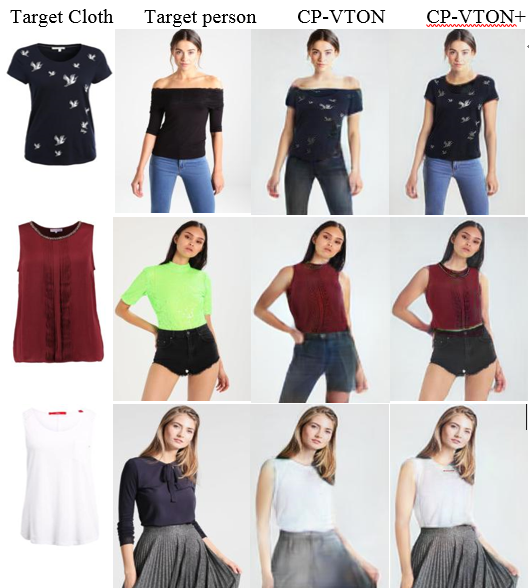
\includegraphics[height=6.5cm, scale=1]{figures/cpvton_cpvton+keyresult.png}   % TODO
%\caption{The proposed VTON results}
%\label{fig:cpvton_cpvton+keyresult}
%\end{figure}

  % intro

\section{Classified Performance Evaluation of Image-Based VTON}

\subsection{Image-based VTON algorithms}

In this Section, we started with evaluating the 2D image based VTON algorithms using a try-on cloth and a target human image. The human representation is composed of 1) heat maps for each joints 2) silhouette of human body, and 3) face and skin pixels patches (non-cloth and human identity area). It is assumed that the target human image is pre-processed for a cloth agnostic human representation by a human pose estimation like OpenPose\cite{Cao2018OpenPoseRM} and human parsing like LIP \cite{Liang2018LookIP}. % the algorithms 
We use the same dataset collected by Han et al. used in VITON\cite{Han2017VITONAI} and CP-VTON\cite{Wang2018TowardCI} papers. Here we include the SCM based-VTON, VITON \cite{Han2017VITONAI}, and  CP-VTON \cite{Wang2018TowardCI}. We included the SCM based algorithm  for a representative of non deep learning algorithm.

For clear notation, $C_i \in R^{H \times W \times3} $ denotes the try-on input cloth image 
and $ H_t = (J_t, R_t, S_t)$ is a human representation, 
where $ J_t \in R^{H \times W \times J}$, $R_t \in R^{H \times W \times 3}$, and $ S_t \in R^{H \times W}$ are a joint heat-map, residual (e.g hands, faces, hairs) color pixel images, and body shape silhouette merged human parsing segmentations from a human image $I_i$, respectively.    

The previous algorithms are mostly composed of two stages: (1) cloth warping step that warps the try-on cloth to align with the pose and shape of the target model (called GMM in CP-VTON \cite{Wang2018TowardCI}: geometric Manipulation Module), and (2) blending step that blends the warped cloth onto the target human image (called TON in CP-VTON: Try-On Network). 

The cloth warping step is done using SCM matching and transform from try-on cloth to the current, target cloth segmentation area, and the final VTON image is blended using simple alpha blending. For VITON and CP-VTON, a brief summary is as follows. For more details, the reader is refer to the original papers.


GMM of SCM-based VTON is defined by  
$
   \bold{\theta} = f_{SCM} (C_t, C_i)
$
and
$
   C_{warped} = f_{TPS}(\theta, Ci)
$.    
GMM of VITON is defined by 
$
   (I_{r}, M_{warped}) = f_{\theta, VITON} (H_t, C_i) 
$
and the loss function for training, 
\[
   L_{GMM}^{VITON} =   \sum_{i=0}^{5} \lambda_i || \phi (I_r) - \phi (I_i)||  + 
   ||M_{C_{warped}} -  M_{C_t}||_1 .
\]
GMM of CP-VTON, GMM is defined by 
$  
   \bold{\theta} = f_{\theta} ( f_H (H_t), f_C(C_i) )
$
and
$
   C_{warped} = f_{TPS}(\theta, Ci).
$    
with the training loss function
\[
   L_{GMM}^{CP-VTON} =  \sum ||C_{warped}, C_t||_1
\]

% GMM
The VITON use an encoder-decoder network to generate the warped cloth mask. Then the estimated TPS parameter from SCM matching between the generated mask and input try-on cloth mask is applied to the input try-on cloth. This is because in general the generated images from an encoder-decoder network does not preserved the original cloth as well as the warped image by geometric transform. Instead, CP-VTON uses a CNN based correlation network to estimated the TPS parameter directly and use the estimated parameters for warping.   


TOM  of SCM-based VTON  is defined by 
$
   M = f_{TPS}(\theta, M_{Ci}),
$    
and 
$
   I_o = M \odot C_{warped}, + (1-M) \odot I_i 
$.
TOM of VITON is defined by 
$
   \bold{\theta} = f_{SCM} (M_{C_t}, M_{C_i})
$,
$
   C_{warped} = f_{TPS}(\theta, Ci)
$,    
$
 M = f_{TOM} ( I_{r1}, C_{warped} ) 
$, 
and 
$
   I_o = M \odot C_{warped}, + (1-M) \odot I_{r},
$
with the training loss function, 
\[
   L_{TOM}^{VITON} = \lambda_{VGG} \sum_{i=3}^{5} \lambda_i || \phi_i(I_o) - \phi_i(I_t)||_{1}  + 
             \lambda_{warp}  || M ||_{1}  + 
             \lambda_{TV} || \nabla M||_{1}      
\]
TOM of CP-VTON is defined by 
$
 (M, I_r) = f_{TOM} ( H_t, C_{warped} )  
$
and 
$
   I_o = M \odot C_{warped} + (1-M) \odot I_r
$
with the training loss function, 
\[
   L_{TOM}^{CP-VTON} = \lambda_{L1}  || I_o - I_t ||_1  + 
             \lambda_{VGG} \sum_{i=1}^{5} || \phi_i(I_o) - \phi_i(I_t)||_1  + 
             \lambda_{mask} || 1 - M ||_1      
\]


% TOM
In TOM, the blending step, VITON generates an alpha blending mask image, which is used when alpha-blended with warped try-on cloth and human input image. The authors of CP-VTON observed that the blending is not successful when the warped  cloth area does not align well with the target area of human image, and first generates a coarse VTON results in addition to the composition mask, and then alpha-blends the warped cloth and the coarse VTON image with the alpha-composition mask.       


Differently from other GAN applications where the main purpose is to generate an unseen, plausible image, VTON application needs to retain the original texture and shape of the input try-on cloth. Due to its higher performance and logical architecture, CP-VTON \cite{Wang2018TowardCI} has become the benchmark benchmark algorithm for the image-based VTON algorithms recently published 
% \cite{     }.  But we can not include them in this paper because the implementations are not available. However, we believe the works share the strength and problems with three algorithms examined here. 


%The previous and following in 2019 share same input image and information conditions with CP-VTON and compare the results with it.
% Add some paper summary after CP-VTON .... and explain the differences from our works.

 
\subsection{Sample Classification}

% The criteria for classification   
First of all, the criteria for classifying the experimental samples were divided into the complexity of try-on cloths and the degree of occlusion (OP, OB, OF), posture (P), and shape (S) of the target cloth area of the human images. For the complexity of try-on cloths, we only uses two groups: long sleeved vs short sleeved, because the length of sleeves is the biggest component in cloth warping and the dataset does not have full styles.    


%The degree of obscuration is a factor that affects the accuracy of the object of deformation, the posture is the degree of deformation, and the complexity of the clothes means the processing complexity of the clothes themselves.
%However, it is included in the range of classification, but not included in the actual experiment is shown in parentheses. Excluded conditions are those that are not included in the test data or that the evaluation is considered to be complex in the current technology. Based on this, six cases were classified as follows.

\begin{itemize}

\item[$\bullet$] B:  no or little occlusion and posture (with long sleeve and  short sleeve)
\item[$\bullet$] OP: the target area partly covered by hair and arms
\item[$\bullet$] OB: A large part of the clothing is covered by the bottoms.
\item[$\bullet$] OF: the target area covered by the arms (with long sleeve and short sleeve)
\item[$\bullet$] P:  large posture deformation (e.g. a large movement of the arm or twisted or lateral posture)
\item[$\bullet$] S:  large body shape change  (over-weighted or pregnant)

\end{itemize}

The cloth shape in the VITON dataset are mostly simple in shape and texture, e.g. a T-shirt (without a collar) of  monochromatic or monotone patterns. Even though it is clearly biased dataset, it is also not easy to define the un-biased one. Although all 2023 test images are used for experiment, some categories, e.g. S, does not have only small samples. But the trends of results in each category are very clear. 


For evaluation of performance, we used same cloth re-try on and new cloth try-on. 
The same cloth re-try-on experiment are done for quantitative evaluation of the algorithm with the ground truth results. 

\subsection{Same Cloth Re-Try-On Result} 

In the same clothing experiment, we evaluate GMM step performance using IoU (intersection over union) and TOM step performance using average SSIM (Structured Similarity Index).

\begin{equation}
 IoU = \frac{ \hat{M}_{warped} \cap M_{cloth}}
            { \hat{M}_{warped} \cup M_{cloth}}
\end{equation} 


\begin{equation}
 SSIM = \frac{ ( 2 \mu_x \mu_y + c_1 )(2 \sigma_{xy} + c_2) }
             { ( \mu^2_x + \mu^2_y +c_1) ( \sigma^2_x + \sigma^2_y + c_2)}
 \end{equation} 

\begin{itemize}

\item[$\bullet$] B: All three algorithms show higher performance for short-sleeve cloth. In particular, SCM-based shows high performance. However, for long arms, the deformation of the arm was not good. This result shows the matching and deformation are mainly done globally based on the whole silhouette, but not optimized for local deformation at sleeve area. TOM stage in VITON and CP-VTON hides some degree of mis-alignment by blending the un-covered target cloth area.   %Including the skeletal information can be supplemented, but at present, no algorithm has been developed for automatically extracting the skeletal information of the garment.

\item[$\bullet$] OP: Partial occlusion by hair and other parts, cause wrong target cloth area and human silhouette. All three algorithms affected this strongly. Therefore, it is expected to improve the GMM part by removing elements such as hair and using only body shapes.

\item[$\bullet$] OB: Occlusion due to bottoms occurs. SCM algorithm does not distinguish between deformation and occlusion and use the target cloth area directly for deformation parameter estimation.  Therefore, GMM results show unnatural deformation especially for long cloths. Since VITON and CP-VITON use silhouette from cloth-agnostic human representation, this effect are reduced.

\item[$\bullet$] OF: TOM of all three algorithms are confused in deciding whether the arm area should covered by cloth or skin color, especially when the new cloth's sleeve length are different from the current cloth's.  

\item[$\bullet$] P: All three algorithms have a big error in the clothing deformation. This is considered to be a big limitation using the two-dimensional algorithm.

\item[$\bullet$] S: In VITON dataset, the matching cloth is large for big human images, the effects is not serious for the same cloth re-try-on.
\end{itemize}

\subsection{ New Cloth Try-On Results }
 
The wearing of a new cloth is, in effect, the ultimate result of the application. As above, objective evaluation is not possible with VITON dataset. Therefore we compare the relative differences of each algorithm based on visual observations.

\begin{itemize}

\item[$\bullet$] B: The clothing deformation itself shows good results similar to the result with same cloths, but there are some differences according to the algorithms in the synthesis. When switching from long to short sleeves, SCM does not restore the skin area, whereas VITON and CP-VTON can generate the skin area for the revealing bare arm. Especially due to the coarse VTON output of it, CP-VTON can generate much clear skin area.

\item[$\bullet$] OP: The performance was similar to that of the same clothes.

\item[$\bullet$] OB: The same characteristics as the same image, that is, the SCM shows a problem that can not distinguish between the mask and deformation.

\item[$\bullet$] OF: The same characteristics as the costume. Here too, in the case of SCM, the synthesis algorithm needs to be improved when switching from short arm to long arm.

\item[$\bullet$] P: As in the case of the same costume, there was a large error in deformation.

\item[$\bullet$] S: Results shows GMM, especially of VITON and CP-VTON, can warp the new cloth to the target human body shape change, 

\end{itemize}

%In addition to the analysis of each condition in addition to the analysis of each condition, it can be seen that there are the following big features. First, it was confirmed that the shape change of clothes by GMM has an influence on the current wear clothes. The reason is that SCMM uses the area of the current costume, and deep learning methods use the body itself, but the area of the current costume is reflected in the correct answer mask used in the learning process.

 
\subsection{Discussion for Improvement}

% comparison between algorithm
Comparing the performance the algorithms used, CP-VTON show the best quality in both same cloth re-try-on and new cloth try-on. However there are some notable observations. CP-VTON GMM using CNN Geometry matching algorithm shows better results than VITON GMM. The GMM results for the same cloth shows SCM show best quality, which might sound conflicting against the result in \cite{Wang2018TowardCI}. It can be explained that only new cloth case are examined in \cite{Wang2018TowardCI}. whereas SCM can use the ground truth target in same cloth re-try-on.  In the same cloth re-try on, SCM show more reliable results than the current CNN Geometry matching algorithm used in CV-VTON.       
As for TOM stage, VITON generates blurred cloth due to the un-clear composition alpha-map, CP-VTON generated much clear cloth texture, and SCM generates noticeable cloth boundary.     


%All the used image-based algorithms shows similar trends in each input
%Even though the success and failure cases are presented and compared with other algorithms' results, the failure case analysis is not enough for understanding the origin of failure cases and therefore difficult to find the solution for them. A classified evaluation would be better for this understanding. Here we summarized the classified results from our another study. We classify input try-on cloth and target human images according to the posture and body type of the person, the degree of occlusion of the clothes, and the characteristics of the clothes. Quality is compared in IoU for the warping step and in SSIM for the final blending step for same cloth re-try-on cases. We also tested for the new cloth try-on cases but did not include here for limitation of spaces, and the same cloth cases are enough to explain the tendencies of the performances. Though in general CP-VTON generates the best quality image, the relative comparison is not the main purpose of the analysis. Please refer to Figure \ref{fig:classified2DVTONresult} for detailed results.


\begin{figure}
\centering
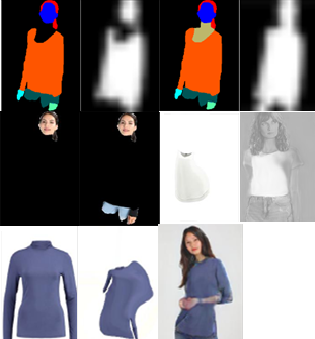
\includegraphics[height=8.5cm, scale=1]{figures/cpvtonissues.png}   % TODO
\caption{The issues in CP-VTON}
\label{fig:cpvtonissues}
\end{figure}

% 1.
Firstly, even though they argued and tried to use cloth-agnostic human representation, the current VITON target try-on area is dependent upon current cloth shape. Especially, the neck area pixels are labeled as background and some body areas are occluded by hairs or accessories (Figure \ref{fig:cpvtonissues}), which affects in cloth warping and blending. 
% 2.
Secondly, all the unintended part, faces, bottom-clothes and legs have to be preserved in blending stage. But other parts except face and hair are missing in CP-VTON\cite{Wang2018TowardCI} human representation and generated at blending stage, which is all right for general synthesis application but not desirable in VTON application (Figure \ref{fig:cpvtonissues}). 
% 3.
Thirdly, the texture is often not vivid, which is due to the composition. Examining the original loss function of TOM network, the term for the composition alpha mask are poorly formulated as simple regularization loss.   

\begin{equation}
L = \lambda_{L1} || I_0-I_{GT} ||_1 +  \lambda_{VGG} L_{VGG}+ \lambda_3 || 1 - M_{o} ||_1        
\end{equation} 

%4. 
Fourthly, since no label in the area of warped cloth is the same color as background, white colored clothes are confused and improperly processed in the blending stage (Fig. 3 (c))


Finally, GMM module using Spatial Transform Network\cite{JaderbergSZK15} with TPS (Thin Plate Spline)\cite{Bookstein1989PrincipalWT} deformation cannot handle strong 3D deformation due to the target pose and also generates artifacts because of the person representation inputs. For example, hands-up and folded arms.  Note that many errors in the warping stage are often hidden in the blending stage when the target clothes are single-colored, which can be expected in practical conditions 
%(Fig. 3 (d)).


%Especially note that the warped cloth are often too much different for desired shape. It is originated two facts. First the 3D deformation that any 2D deformation including non-rigid transform such as TPS is quite limited, especially any 2D deformation cannot handle when the two area in the original image are overlapped in the destination images. There for when the arms of long sleeved cloth occlude the main body, 2D warping cannot approximate the 3D deformation properly. Second, the deformation needs corresponding points  between the source nd target image. The cloth are extremely difficult object to find the corresponding points. The STN (spatial transform network)\cite{JaderbergSZK15} and SCM (shape context matching)\cite{BelongieMP02} cannot find the corresponding points when the target cloth and original cloth has different shapes. In conclusion, the 2D image based algorithm has serious limitation in the range of applications. It can apply to the mild posed target human only and simple short sleeved cloth, mainly because the inherent limitation of 2D deformation method including non-rigid ones, and the poor performance of matching algorithm.  To overcome this limitation, we consider to model the try-on cloth into 3D model and apply the 3D deformation

\begin{figure}
\centering
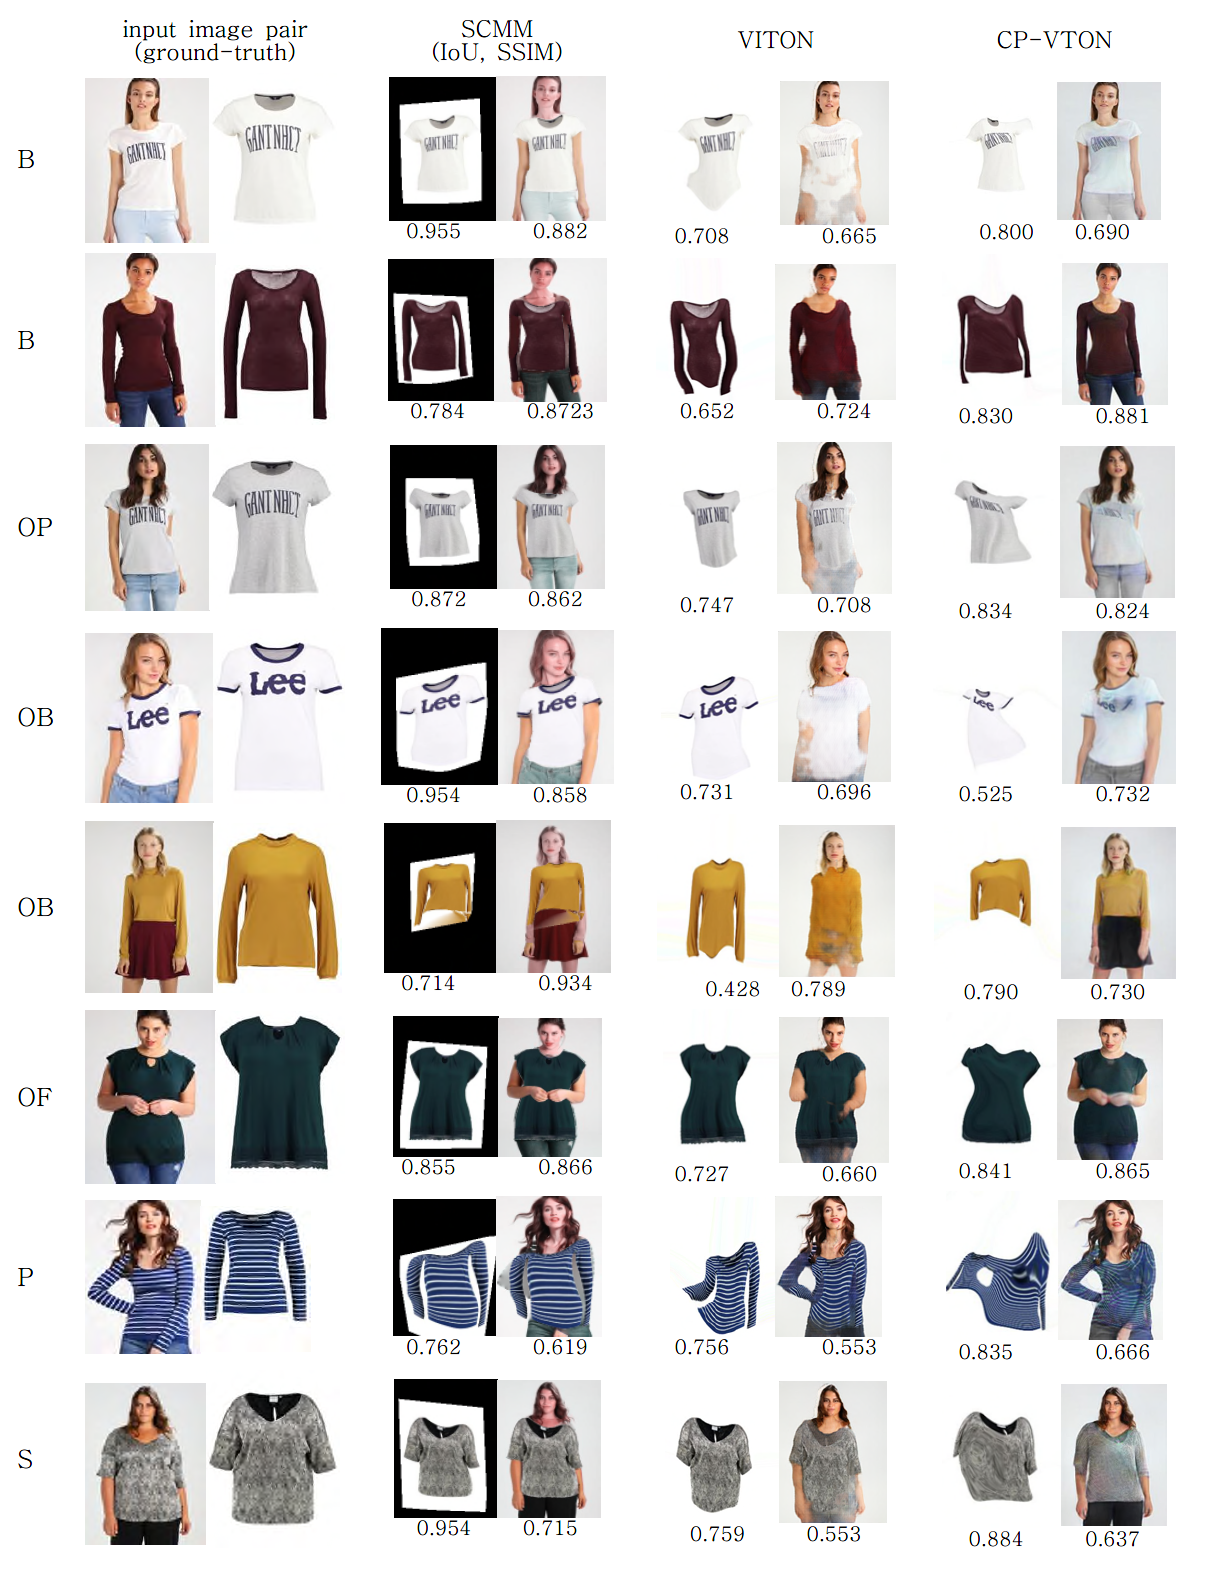
\includegraphics[height=13.5cm, scale=1]{figures/2dvton_same.png}   
\caption{Classified Evaluation of Image-based VTONs (same cloth re-try-on)}
\label{fig:2dvton_same}
\end{figure}

\begin{figure}
\centering
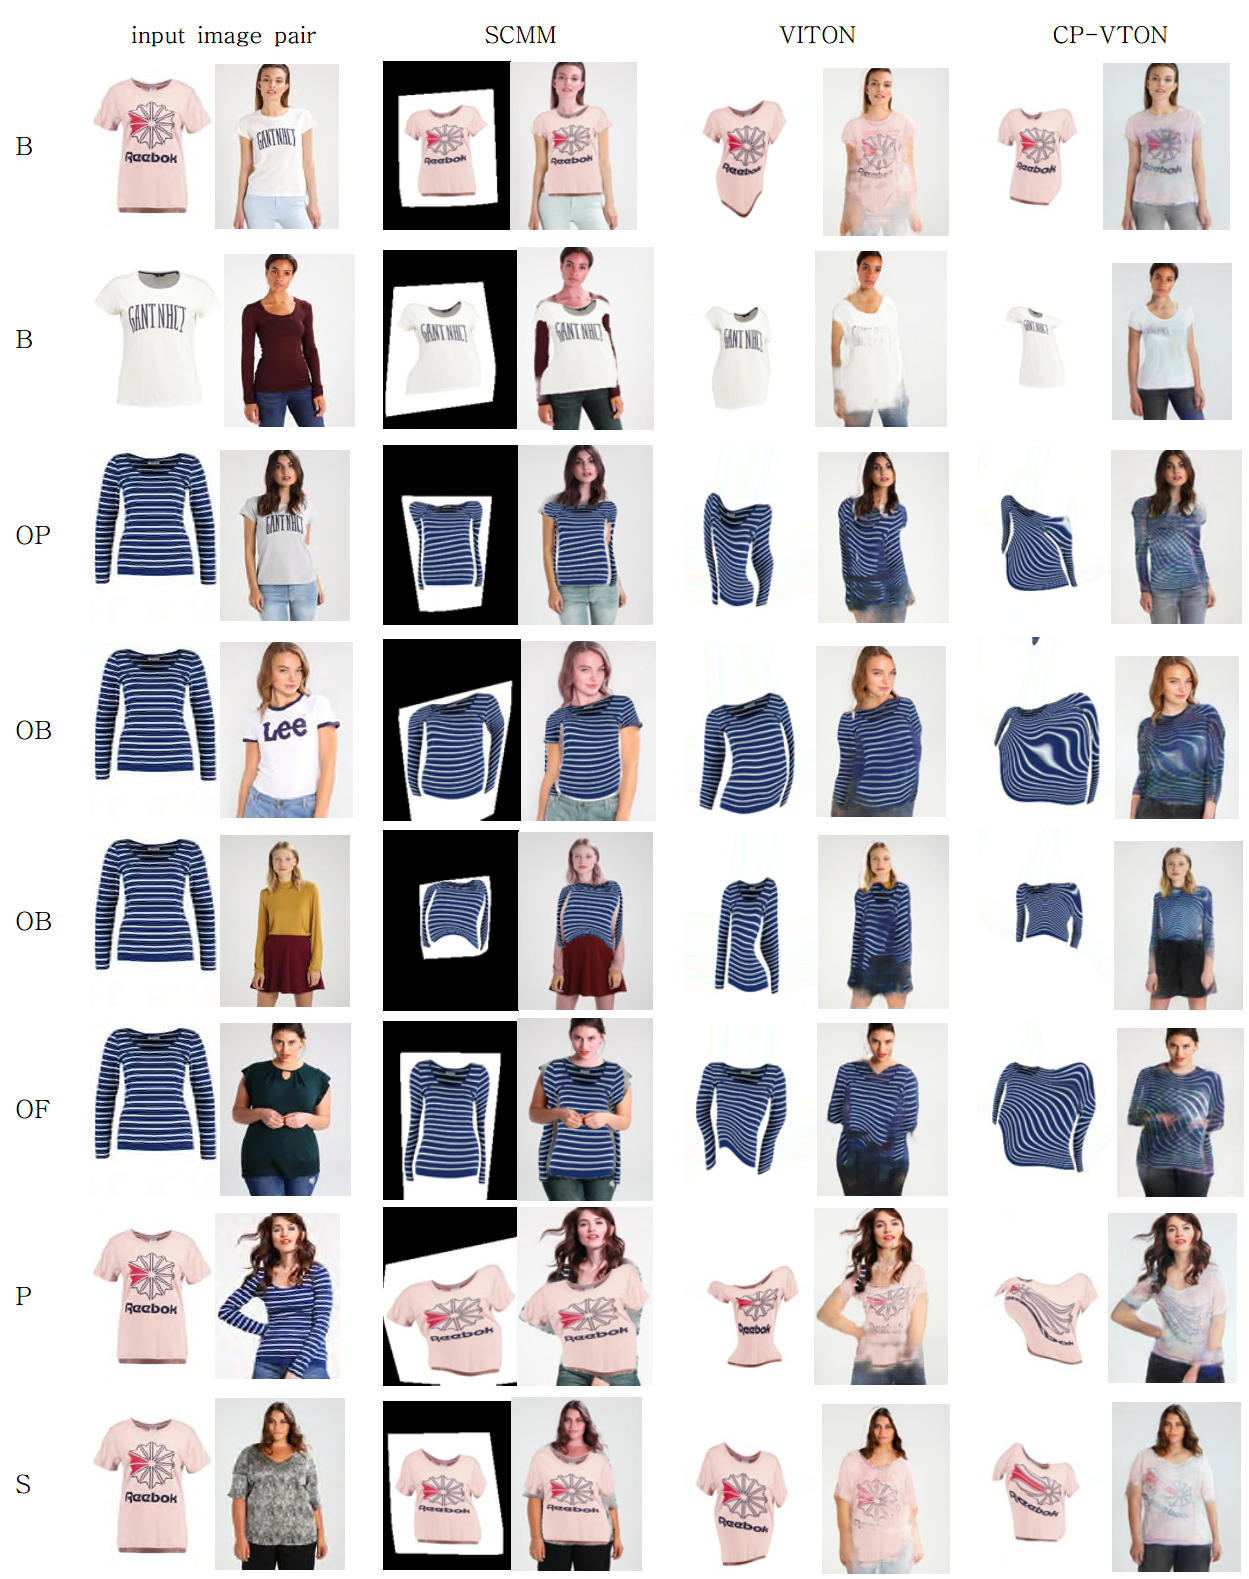
\includegraphics[height=13.5cm, scale=1]{figures/2dvton_diff.png}  %% TODO  
\caption{Classified Evaluation of Image-based VTONs (new cloth try-on)}
\label{fig:2dvton_diff}
\end{figure}
  % Classified analysis
\section{CP-VTON+} \label{section:cpvton+}

\subsection{Overview} 
Based on the experiment results and analysis for problems in the previous work, the new VTON pipeline are designed based on the pipeline structure of CP-VTON, hence named CP-VTON+. Fig. \ref{fig:piepline} illustrates the architecture with highlighting the upgraded components for comparison. The details are described as follows.

\begin{figure}[t]
\centering
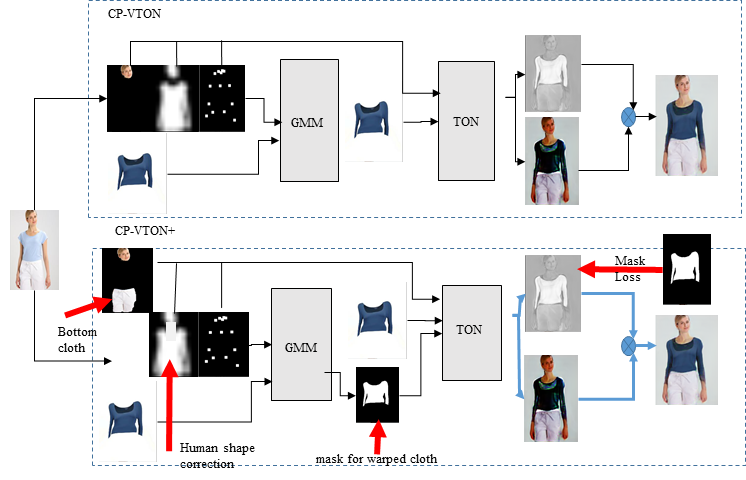
\includegraphics[height=6.5cm, scale=1]{figures/cpvton+pipeline.png}   
\caption{Full pipeline Comparison: CP-VTON and CP-VTON+: TODO: UPDATE with some more detailed one!!!}
\label{fig:piepline}
\end{figure}

\subsubsection{Cloth Warping Stage}

The modification in GMM stage are three locations. 
% Correction on the cloth agnostic human representation:
First, It is crucial to obtain the complete target body area for the try-on cloth and the target area should be the current-cloth agnostic. As described above, the original VITON dataset does not satisfy this requirement. We define a segmentation correction process as follow.  
% BG2SKIN
To be independent upon the current cloth the human wear, a new label ‘skin’ is added to the label set, and then  the pixels wrongly labeled as 'background' in VITON dataset are replaced by 'skin' considering the joint locations. The skin-labeled area now is included in the silhouette in the human representation (Figure  ~\ref{fig:cpvtonissues} (a)).
% HAIR-OCCLUSION
To recover the hair occlusion over the body, first the hair occlusion area are identified as the intersection of convex contour of the upper cloth and the hair-labeled area, and the intersection are re-labeled as upper cloth.   
% @TODO!!
%\ref{fig:cpvtonissues} (a)).

% GIC Network modification: 
Second, CP-VTON GMM network is built on CNN geometric matching \cite{rocco2017convolutional}, and trained in self-supervised manner by the L1 loss between the warped cloth images and the current human cloth. It is quite interesting that CNN geometric matching uses a pair of color images, but CP-VTON GMM uses a human representation, e.g. silhouette and joint heatmap with the try-on cloth. The texture information from try-on cloth does not help in matching process, thus our GMM use $M_{C_i}$ instead of $C_i$, i.e.,  
\[  
   \bold{\theta} = f_{\theta} ( f_H (H_t), f_C(M_{C_i}) )
\]
%The human representation only provide the shape and structure information 
%and the try-on cloth provides both texture and shape information. 


Finally, the experiments above reveals the warped cloth often distorted severely. We tried to understand the origin of this distortion, but it is not easy to explain clearly.  However, we conclude that the TPS parameter estimation needs the regularization, taking into account the restriction of cloth textile. Our grid warping regularization is defined on the grid deformation not directly the TPS parameter for easy visualization and understanding,  not to have too much different warping from the before and next grid gap in equation ~\ref{eq:gridloss}.
\begin{equation}
 L_{GMM}^{CP-VTON+}  = \lambda_1 \cdot L1(C_{warped}, I_{C_t}) + lambda_2 \cdot  L_{reg}  
\end{equation}

%The comparison result \cite{fig:2dvton_same} and \cite{fig:2dvton_diff} shows the 


%, which again uses the spatial transform networks by Zimmerman et al.'s \cite{jaderberg2015spatial}. Although warping network can work in both instance-level and category-level, our experiments  reveals the warped cloth often distorted severely.


%Our finding is that the warping network try to matches cloth images with human representation of silhouette and joint heatmap. The latter does not have no texture features but the shape information. From the failure case examinations, we found that the warping in the failure case is often too extreme, so that we try to restrict the warping parameters. Instead of single step TPS warping, we designed 2 stage warping network, in the first stage it warped roughly with Affine transform, and in the second stage it warped delicately with TPS transform. Not to have un-realistic warping, we added warping regularization loss. In the second stage, the sizes of cloth and target area in the human representation are in the same scale, so that the matching network can find the matching better. 


\begin{equation}\label{eq:gridloss}
\begin{aligned}
 L_{reg} (G_x, G_y) = \sum_x \sum_y | G_x(x+1, y) - G_x(x, y) | - | G_x(x, y) - G_x(x-1, y) | \\
 + | G_y(x, y+1) - G_y(x, y) | - | G_y(x, y) - G_y(x, y-1) |
\end{aligned}
\end{equation}



\subsubsection{Blending Stage}

The modification to GMM stage are two locations.
%\begin{itemize}
%\item[$\bullet$] Retaining the remaining area except the target cloth  :
In order to retain the other human components except the target cloth area, e.g. bottom clothes and legs, the all other area except the target cloth area are added for the human representation input of TOM, along with face and hair (Figure ~\ref{fig:cpvtonissues} (c))

%\item[$\bullet$] Training Composition alpha-map:  
In the mask loss term in TOM loss function, we replaced the Composition Mask with supervised ground truth mask for a strong alpha mask.

\begin{equation}
 L_{TOM}^{CP-VTON+} = \lambda_{L1} || I_0-I_{GT}||_1+  \lambda_{VGG} L_{VGG} + \lambda_{mask} ||M_{GT}-M_o||_1       
\end{equation}

Also, we added the binary mask of warped cloth to TOM network input so that TOM can clearly differentiate the target cloth area regardless of cloth color.  

%\end{itemize}

%\begin{figure}
%\centering
%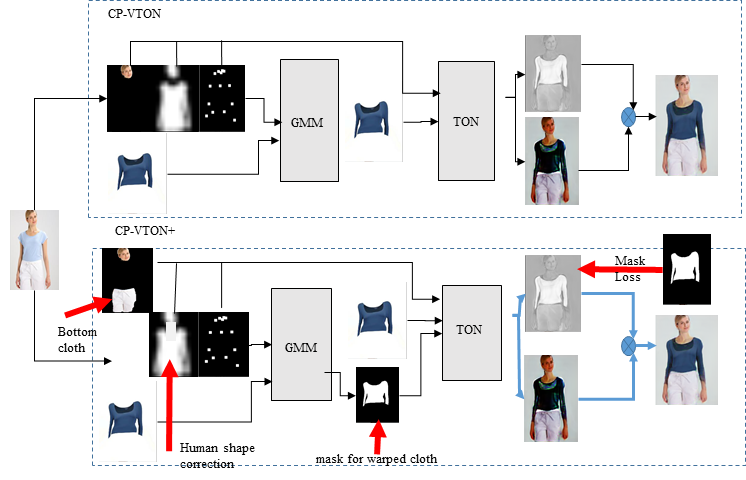
\includegraphics[height=6.5cm, scale=1]{figures/cpvton+pipeline.png}   
%\caption{2 stage GMM design with regularization loss}
%\label{fig:piepline}
%\end{figure}

  % CPVTON+ 
\section{Experiment and Results} 

\subsection{Implementation details} 

For CP-VTON+ network implementation is based on CP-VTON PyTorch and extended the network as described above. We also used the modified human image segmentation and human representation. The network  For training, we refer \cite{Wang2018TowardCI} and used similar setting for comparison. We used $L_1 = L_{vgg} = L_{mask} =1$ and $L_{reg} = 0.5$ through  hyper-parameter tuning. We trained both networks for 200K steps with batch size 4 with Adam optimizer with $\beta_1 = 0.5$ and $\beta_2 = 0.999$. Learning rate is first fixed at $0.0001$ for 100K steps and then linearly decays to zero for the remaining steps. 

\subsection{Comparative Results}

To evaluate the performance improvement of CP-VTON+, we compare the performance with CP-VTON, since CP-VTON shows the best performance in the previous research and our in-depth comparison study.

VITON cloth-human pair dataset is again used for training and test dataset. We used IoU and SSIM performance metrics for the same cloth retry-on cases for warping stage and blending stage, respectively. The original target human image is used for the reference image for SSIM and the parsed segmentation area for the current top cloth is used for IoU reference. Our proposed method, CP-VTON+ outperforms CP-VTON all measures: in IoU  with  0.8325 over o.7883 (around 7 $\%$)and in SSIM with 0.8163 over 0.7798 (around 5 $\%$). The performance improvement in warping stage is lager than final results. 
Since SSIM is originally developed for geometrically aligned image comparison, Learned Perceptual Image Patch Similarity (LPIPS) metric \cite{zhang2018unreasonable} measure is added to evaluate the deep learning visual similarity. CP-VTON+ outperforms CP-VTON in LPIPS with 0.1263 over 0.1397.

% TODO check smaller is better???


%Special comments are required for the IoU values, where CP-VTON (0.78) is slightly higher than CP-VTON+ (0.75). The un-expected results originated due to CP-VTON generating as in the current cloth shape. However, similar clothes are not always applicable, furthermore, it generates wrong shaped results for different clothes. Fig. 6 illustrates this with two typical example, plugging and normal tops

For different cloth try-on, Inception Score (IS) is used together with visual examinations. CP-VTON+ outperforms slightly CP-VTON in IS with 2.76 over 2.7417. Figure \ref{fig:2dvton_same} and Figure \ref{fig:2dvton_diff} show the representative results selected for presentation. The subjective evaluation shows significant visual improvements.  1) the warped clothes do not have severe distortion. 2) the bottom clothes are retained. 3) the new cloth collar shape is not affected by the current cloth's collar shape. 4) cloth textures such as logos and patterns are clearer.
 
 
%We added the test results for all test cases for comparison between CP-VTON and CP-VTON+ in supplementary materials, together with the categorized comparison of SCM-based VTON, VITON and CP-VTON

%\begin{figure}
%\centering
%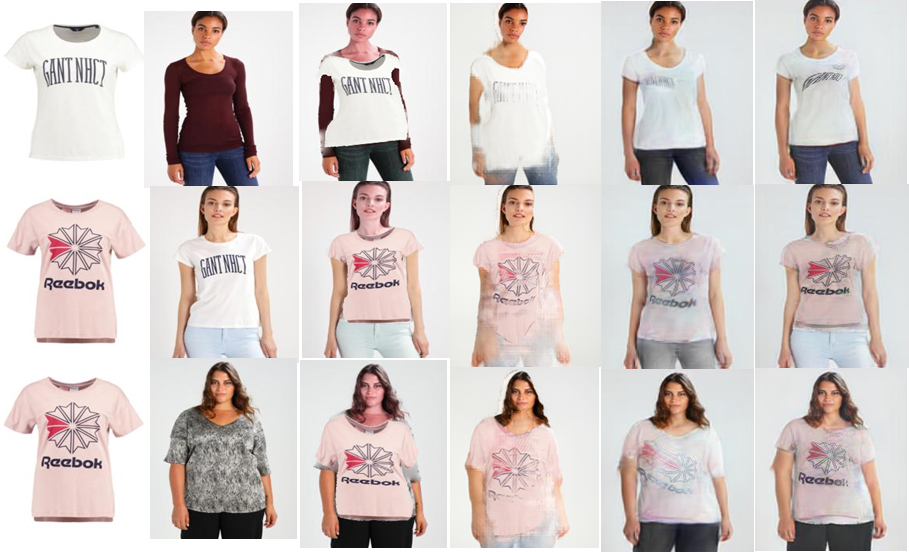
\includegraphics[height=6.5cm, scale=1]{figures/cpvton+compare.png} 
%\caption{VTON results: We have to include 1) %GMM and TOM results for demonstrating all the improvement one by one: }
%\label{fig:vtonresults}
%\end{figure}


\subsection{Ablation Study}

Figure ~\ref{fig:ablation} we highlight the impact of the identified problems and improvement of the proposed method step-by-step through the ablation study of CP-VTON+. The first and second columns are target humans and try-on clothes, respectively. The third column is vanilla CP-VTON results. The fourth column is when unchanged clothes and body parts are added to the reserved region inputs of TOM, retaining the original pants texture. The fifth column is when the mask loss function of TOM is updated with the target cloth area, making the texture and color of cloth sharp and vivid. Finally the sixth and last column is when the body masks are updated, replacing the skin area wrongly labelled as background and hair are removed from the reserved region input of GMM, making GMM can better cloth-and-hair-agnostic human representation.  


\begin{figure}
\centering
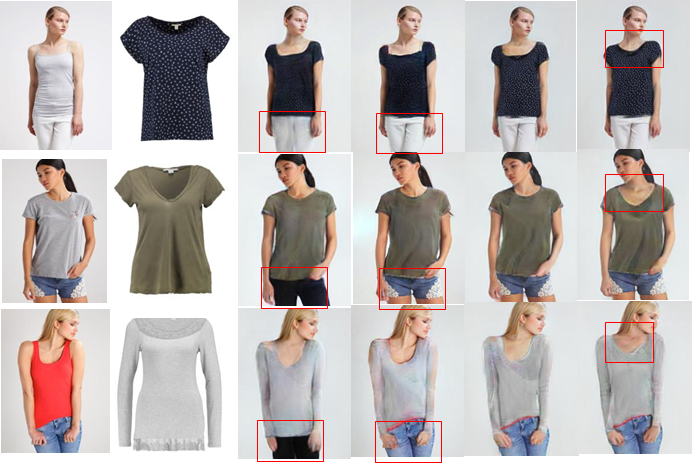
\includegraphics[height=6.5cm, scale=1]{figures/ablation.png} 
\caption{Ablation study of CP-VTON+. From left to right column: target humans, try-on clothes, CP-VTON, with corrected human representation in TOM, warped cloth mask and mask loss function updated, and CP-VTON+ (with corrected human representation in GMM)
}
\label{fig:ablation}
\end{figure}


\subsection{Discussion}

Even though CP-VTON+ improves the quality to some degree, and showing highly natural results, the experiment is still limited because the dataset has limited samples for difficult cases, like the long sleeved, complicated shaped, or textured cloth and large posture target human. 

As Figure ~\ref{fig:gmmfailure} shows two typical failure cases due to the cloth warping. First row shows when the arms heavily covers the body area. The warped cloth does not match to the human body and TON failed in hiding the warping error. 
% STN (Spatial Transform Network). STN is originally developed for invert the (augmented) input images for different camera views and camera distortion.
Any classical 2D transform including on-rigid TPS algorithms, cannot handle the strong 3D deformations of cloth.  Also the 3D poses induce self-occlusions. The TON network should recognized the cloth area and skin areas, like naked arms. One practical short-term solution would be to restrict the pose of target human image from the customer. 

The second rows shows the another problems. Even without strong 3D posture of the target human, the warped cloth often shows un-realistic results. Note that even though the CNN geometric matching argues it can cover the category-level matching. The category is not precisely defined for our application. Mostly the cloth texture can not be used for image feature and the cloth-agnostic human representation does not have even any texture information. Note that the matching algorithm is in fact used without in-depth study on the accuracy for VTON applications. 

    
The output image quality of all image-based VTON algorithms including ours depend upon the quality of input human representation, i.e., estimated joint locations and parsed human segmentation. The poses of target humans are usually (or forced) rather simple so that the state-of-the-art pose estimation algorithms can provide fairly accurate positions. However the quality of parsed human are not always good enough, especially when the target human wear complicated clothes. Also one can restrict the complexity of human images in pose and cloth style, but still the accuracy at the segmentation boundary sometimes affects the blended image results as shown in third row case in Figure ~\ref{fig:ablation}, where the pixels of the current top cloth, which is mislabelled as bottom cloth, remained in the blending result. There fore high quality human parsing algorithm especially around boundaries are required.   

\begin{figure}
\centering
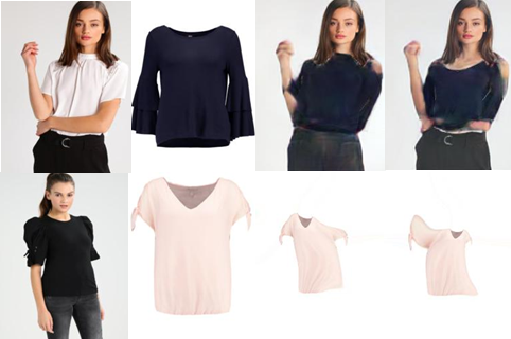
\includegraphics[height=4.5cm, scale=1]{figures/gmmfailure.png} 
\caption{Cloth Warping Failure of CP-VTON+. From left to right column. target humans, try-on clothes, CP-VTON, and CP-VTON+  (Why not same first and second ??)
}
\label{fig:gmmfailure}
\end{figure}
   % Experiments


\section{Conclusions}

Almost all real computer vision algorithms have a certain condition where they work successfully and not. Therefore it is more important than merely developing better algorithms to identify the working condition of algorithms and approaches.  By categorized cloth and human inputs and analysis not only final try-on results but also intermediate results of the pipeline, e.g. the warped cloth, we showed the key successful and unsuccessful conditions and origins of a typical image-based VTON algorithm, CP-VTON. 

With these identified issues, a CP-VTON+, an improvement to CP-VTON was proposed, which produces significant quality improvements over existing state-of-the-art algorithm, CP-VTON. 

However, there remains several areas that we could not yet solved. The automatic warping to the target human shape is still challenging in feature point search and matching and limitation of non-rigid 2-D transforms, and the accuracy human parsing  needs to be improved.
  
     
\clearpage
% ---- Bibliography ----
%
% BibTeX users should specify bibliography style 'splncs04'.
% References will then be sorted and formatted in the correct style.
%
\bibliographystyle{splncs04}
\bibliography{cpvton+bib}



\end{document}
